% ============================================================
% TP3 - PARTIE B : CRITERE ORIENTE TERMINAL
% QUESTION B5 : INTRODUCTION D'UNE HYSTERESIS
% ============================================================

% Packages nécessaires dans le préambule du document :
% \usepackage[utf8]{inputenc}
% \usepackage[T1]{fontenc}
% \usepackage[french]{babel}
% \usepackage{amsmath}
% \usepackage{graphicx}
% \usepackage{float}
% \usepackage{booktabs}
% \usepackage{array}

\section{Question B.5 : Introduction d'une hystérésis}

\subsection{Objectif}

L'objectif de cette expérience est d'étudier l'influence de
l'introduction d'une hystérésis sur le mécanisme de bascule
entre les interfaces LTE et Wi-Fi de l'UE.

Dans la question 3, la décision de bascule repose sur un seuil
unique correspondant au rayon de couverture du point d'accès
Wi-Fi. Cette approche peut provoquer des bascules répétées
lorsque l'UE se déplace à proximité de la limite de couverture.

Afin de limiter ce phénomène, nous introduisons deux seuils
distincts : un seuil d'entrée dans la couverture Wi-Fi et un
seuil de sortie. Nous comparons ensuite le comportement du
système avec et sans hystérésis, en étudiant principalement
le nombre de bascules et la stabilité du débit reçu.

\subsection{Principe de fonctionnement de l'hystérésis}

Soit $R$ le rayon de couverture du point d'accès Wi-Fi et
$H$ la demi-largeur de l'hystérésis.

Les deux seuils sont définis par :

\begin{equation}
    R_{\mathrm{entrée}} = R-H
\end{equation}

\begin{equation}
    R_{\mathrm{sortie}} = R+H
\end{equation}

La décision de bascule dépend alors de la distance $d(t)$
entre l'UE et le point d'accès Wi-Fi :

\begin{equation}
\begin{cases}
\mathrm{LTE} \rightarrow \mathrm{WiFi},
& \text{si } d(t)<R-H \\[5pt]
\mathrm{WiFi} \rightarrow \mathrm{LTE},
& \text{si } d(t)>R+H
\end{cases}
\end{equation}

Lorsque l'UE se trouve entre les deux seuils, l'interface
précédemment sélectionnée est conservée. Cette zone
intermédiaire permet d'éviter les changements d'interface
provoqués par de petites variations de distance autour de
la limite de couverture.

Dans le cas particulier où $H=0$, les deux seuils deviennent
identiques :

\begin{equation}
    R_{\mathrm{entrée}}=R_{\mathrm{sortie}}=R
\end{equation}

Ce cas correspond au mécanisme à seuil unique utilisé dans
la question 3.

\subsection{Protocole expérimental}

Afin de mettre en évidence l'effet de l'hystérésis, nous
conservons le même scénario de mobilité et les mêmes
paramètres de simulation pour les deux configurations.

L'UE suit une trajectoire de type \texttt{border}, qui lui
permet d'osciller autour de la limite de couverture du
point d'accès Wi-Fi. Cette trajectoire est adaptée à
l'étude des bascules répétées.

Le rayon de couverture est fixé à $50$ m et l'amplitude
de déplacement autour de cette limite est fixée à $10$ m.
L'UE se déplace à une vitesse de $5$ m/s pendant une durée
de simulation de $80$ secondes.

Deux configurations sont comparées :

\begin{itemize}
    \item \textbf{Configuration 1 :} absence d'hystérésis,
    avec $H=0$ m.
    \item \textbf{Configuration 2 :} introduction d'une
    hystérésis de $H=5$ m.
\end{itemize}

Les paramètres utilisés sont présentés dans le
tableau~\ref{tab:b5_parameters}.

\begin{table}[H]
    \centering
    \caption{Paramètres de simulation de la question B5}
    \label{tab:b5_parameters}
    \begin{tabular}{|l|c|}
        \hline
        \textbf{Paramètre} & \textbf{Valeur} \\
        \hline
        Type de trajectoire & \texttt{border} \\
        \hline
        Rayon de couverture $R$ & 50 m \\
        \hline
        Amplitude de déplacement & 10 m \\
        \hline
        Vitesse de l'UE & 5 m/s \\
        \hline
        Durée de simulation & 80 s \\
        \hline
        Demi-largeur d'hystérésis $H$ & 0 m et 5 m \\
        \hline
        Seuil d'entrée ($H=0$) & 50 m \\
        \hline
        Seuil de sortie ($H=0$) & 50 m \\
        \hline
        Seuil d'entrée ($H=5$) & 45 m \\
        \hline
        Seuil de sortie ($H=5$) & 55 m \\
        \hline
        Débit nominal & 2 Mbps \\
        \hline
        Shadowing & Désactivé \\
        \hline
        Bruit sur la distance & Désactivé \\
        \hline
        Graine initiale & 1 \\
        \hline
        Numéros de run & 1 à 5 \\
        \hline
        Fenêtre de détection du ping-pong & 15 s \\
        \hline
    \end{tabular}
\end{table}

Cinq exécutions sont réalisées pour chaque configuration,
avec une graine initiale fixée à 1 et des numéros de run
allant de 1 à 5. Le shadowing et le bruit sur la distance
sont désactivés afin d'isoler l'effet de l'hystérésis.

\subsection{Indicateurs de performance}

Les résultats sont évalués à partir des fichiers CSV
générés par la simulation.

\subsubsection{Nombre total de bascules}

Il correspond au nombre total de changements d'interface
entre LTE et Wi-Fi :

\begin{equation}
    N_{\mathrm{switch}} =
    N_{\mathrm{entrée}} + N_{\mathrm{sortie}}
\end{equation}

\subsubsection{Nombre d'événements de ping-pong}

Le ping-pong représente les bascules successives séparées
par un intervalle inférieur à une fenêtre temporelle de
15 secondes.

Une bascule est donc comptabilisée comme un événement de
ping-pong lorsqu'elle intervient moins de 15 secondes
après la bascule précédente.

Cet indicateur permet d'évaluer la fréquence des
changements d'interface rapprochés.

\subsubsection{Stabilité du débit}

La stabilité du débit est évaluée à l'aide du coefficient
de variation (CV), défini par :

\begin{equation}
    CV = \frac{\sigma_{\mathrm{débit}}}
    {\overline{D}}
\end{equation}

où :
\begin{itemize}
    \item $\sigma_{\mathrm{débit}}$ représente l'écart-type
    du débit reçu ;
    \item $\overline{D}$ représente le débit moyen reçu.
\end{itemize}

Le débit est mesuré à partir des compteurs de réception
regroupés dans des intervalles de 100 ms. Pour le calcul
du coefficient de variation, les mesures sont ensuite
agrégées sur des fenêtres successives d'une seconde.

Un CV faible indique une meilleure stabilité du débit,
tandis qu'un CV élevé traduit des variations plus
importantes.

\subsubsection{Proportion du volume reçu via Wi-Fi}

À titre complémentaire, nous considérons la proportion
du volume reçu via Wi-Fi :

\begin{equation}
    P_{\mathrm{WiFi,Rx}} =
    \frac{V_{\mathrm{WiFi,Rx}}}
    {V_{\mathrm{WiFi,Rx}}+V_{\mathrm{LTE,Rx}}}
\end{equation}

Cet indicateur correspond au champ \texttt{offloadRx}
généré par le programme. Il représente la proportion
des octets reçus via Wi-Fi et ne doit pas être confondu
avec le taux d'offloading basé sur le volume transmis.

\subsection{Résultats expérimentaux}

Les cinq exécutions de chaque configuration ont produit
les mêmes nombres de bascules, les mêmes nombres
d'événements de ping-pong et les mêmes proportions de
trafic reçu via Wi-Fi.

Les résultats obtenus sont présentés dans le
tableau~\ref{tab:b5_results}.

\begin{table}[H]
    \centering
    \caption{Comparaison des résultats avec et sans hystérésis}
    \label{tab:b5_results}
    \resizebox{\textwidth}{!}{
    \begin{tabular}{|l|c|c|}
        \hline
        \textbf{Indicateur}
        & \textbf{Sans hystérésis ($H=0$)}
        & \textbf{Avec hystérésis ($H=5$)} \\
        \hline
        Nombre moyen de bascules
        & $20 \pm 0$ & $19 \pm 0$ \\
        \hline
        Nombre moyen de ping-pong
        & $19 \pm 0$ & $18 \pm 0$ \\
        \hline
        Proportion reçue via Wi-Fi
        & 51,28 \% & 50,00 \% \\
        \hline
        Débit moyen
        & 2,000 Mbps & 2,000 Mbps \\
        \hline
        Coefficient de variation (CV)
        & 0,00844 & 0,00846 \\
        \hline
        Taux de pertes
        & 0 \% & 0 \% \\
        \hline
        Délai moyen
        & 9,184 ms & 9,397 ms \\
        \hline
        Délai maximal
        & 22,731 ms & 22,731 ms \\
        \hline
        Durée d'interruption mesurée
        & 0 s & 0 s \\
        \hline
    \end{tabular}
    }
\end{table}

\subsection{Analyse et interprétation des résultats}

\subsubsection{Effet sur le nombre de bascules}

Sans hystérésis, le système effectue en moyenne
20 bascules pendant la simulation.

Avec une hystérésis de 5 m, ce nombre diminue à
19 bascules.

La réduction relative est donnée par :

\begin{equation}
    \frac{20-19}{20}\times100 = 5\%
\end{equation}

Cette diminution montre que l'introduction de deux
seuils distincts limite légèrement les changements
d'interface.

Les fichiers \texttt{switches.csv} confirment également
le déplacement des seuils de bascule :

\begin{itemize}
    \item Sans hystérésis, les transitions LTE vers Wi-Fi
    se produisent à des distances comprises approximativement
    entre 47,5 et 49,5 m. Les transitions Wi-Fi vers LTE
    se produisent entre 50 et 52 m.

    \item Avec hystérésis, les transitions LTE vers Wi-Fi
    se produisent entre 42,5 et 44,5 m, tandis que les
    transitions Wi-Fi vers LTE se produisent entre
    55 et 57 m.
\end{itemize}

Ces valeurs sont cohérentes avec les seuils théoriques
de 45 m et 55 m. Les écarts observés s'expliquent par
la période d'évaluation du mécanisme de décision,
qui est de 0,5 seconde.

% Figure 1 : Nombre de bascules
\begin{figure}[H]
    \centering
    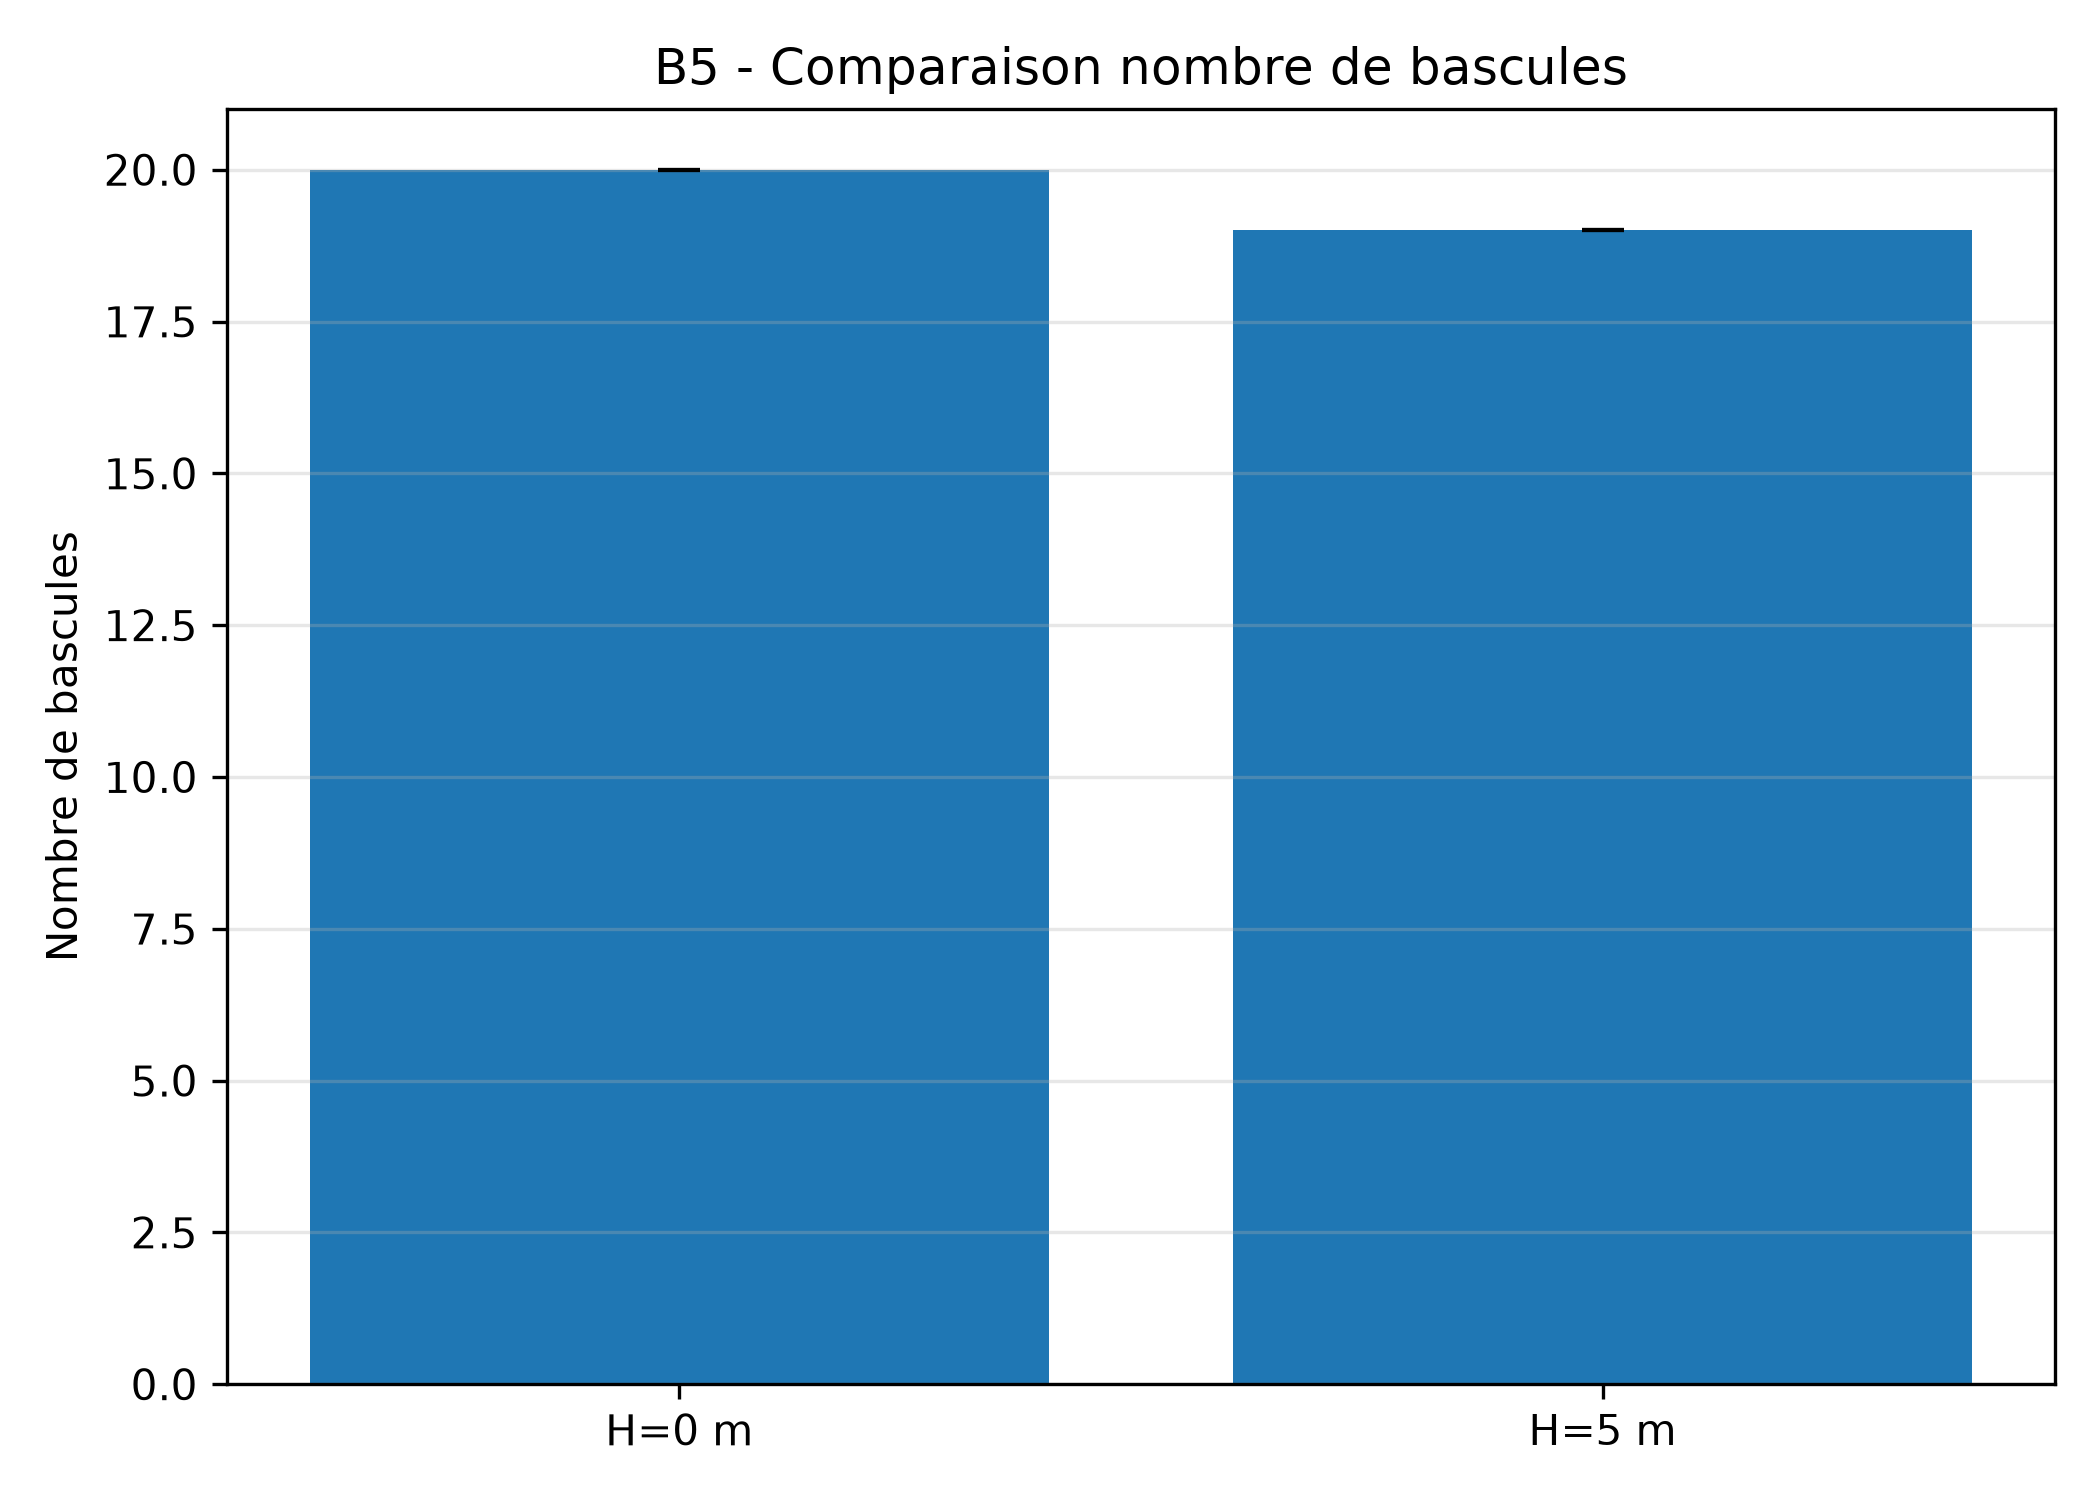
\includegraphics[width=0.85\textwidth]
    {img/B/B5_switches.png}
    \caption{Comparaison du nombre de bascules avec et sans hystérésis.}
    \label{fig:b5_switches}
\end{figure}

\subsubsection{Effet sur les événements de ping-pong}

Le nombre d'événements de ping-pong passe de 19 sans
hystérésis à 18 avec hystérésis.

La réduction relative est :

\begin{equation}
    \frac{19-18}{19}\times100
    \approx 5,26\%
\end{equation}

Cette diminution confirme que l'hystérésis réduit
légèrement les changements d'interface rapprochés.

Cependant, la différence reste limitée dans le
scénario étudié.

% Figure 2 : Evénements de ping-pong
\begin{figure}[H]
    \centering
    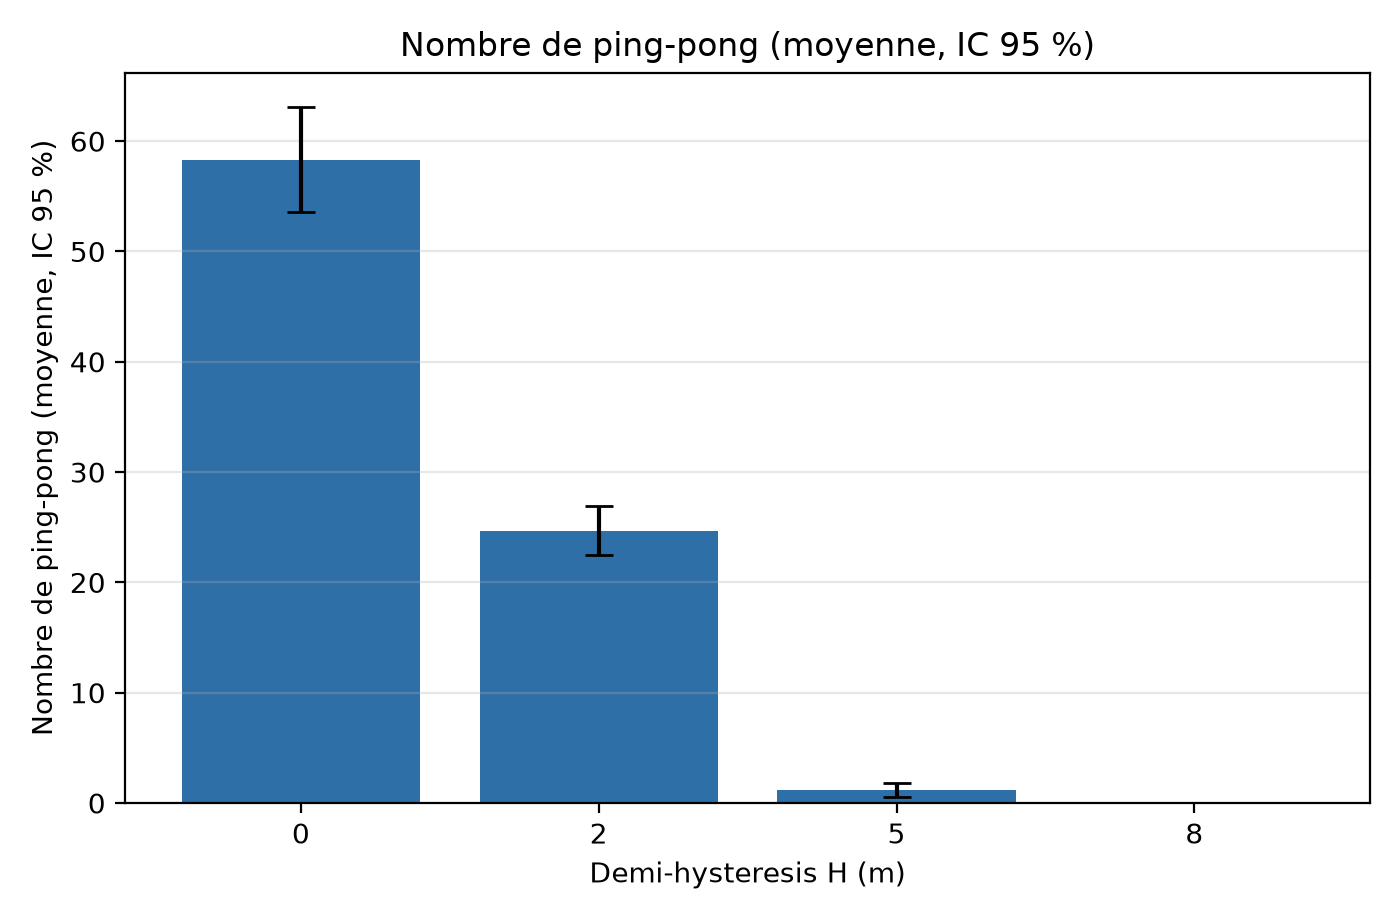
\includegraphics[width=0.85\textwidth]
    {img/B/B5_pingpong.png}
    \caption{Comparaison du nombre d'événements de ping-pong.}
    \label{fig:b5_pingpong}
\end{figure}

\subsubsection{Effet sur la stabilité du débit}

Le débit moyen reste identique dans les deux
configurations :

\begin{equation}
    \overline{D}_{H=0}
    =
    \overline{D}_{H=5}
    =
    2\ \mathrm{Mbps}
\end{equation}

Le coefficient de variation passe de 0,00844 à 0,00846.

Cette légère augmentation indique que la dispersion
relative du débit n'a pas diminué avec l'introduction
de l'hystérésis. La différence observée reste toutefois
très faible et ne permet pas de conclure à une
dégradation significative de la stabilité.

Ainsi, dans cette configuration, l'hystérésis réduit
légèrement le nombre de bascules, mais ne produit pas
d'amélioration mesurable de la stabilité du débit.

% Figure 3 : Coefficient de variation du débit
\begin{figure}[H]
    \centering
    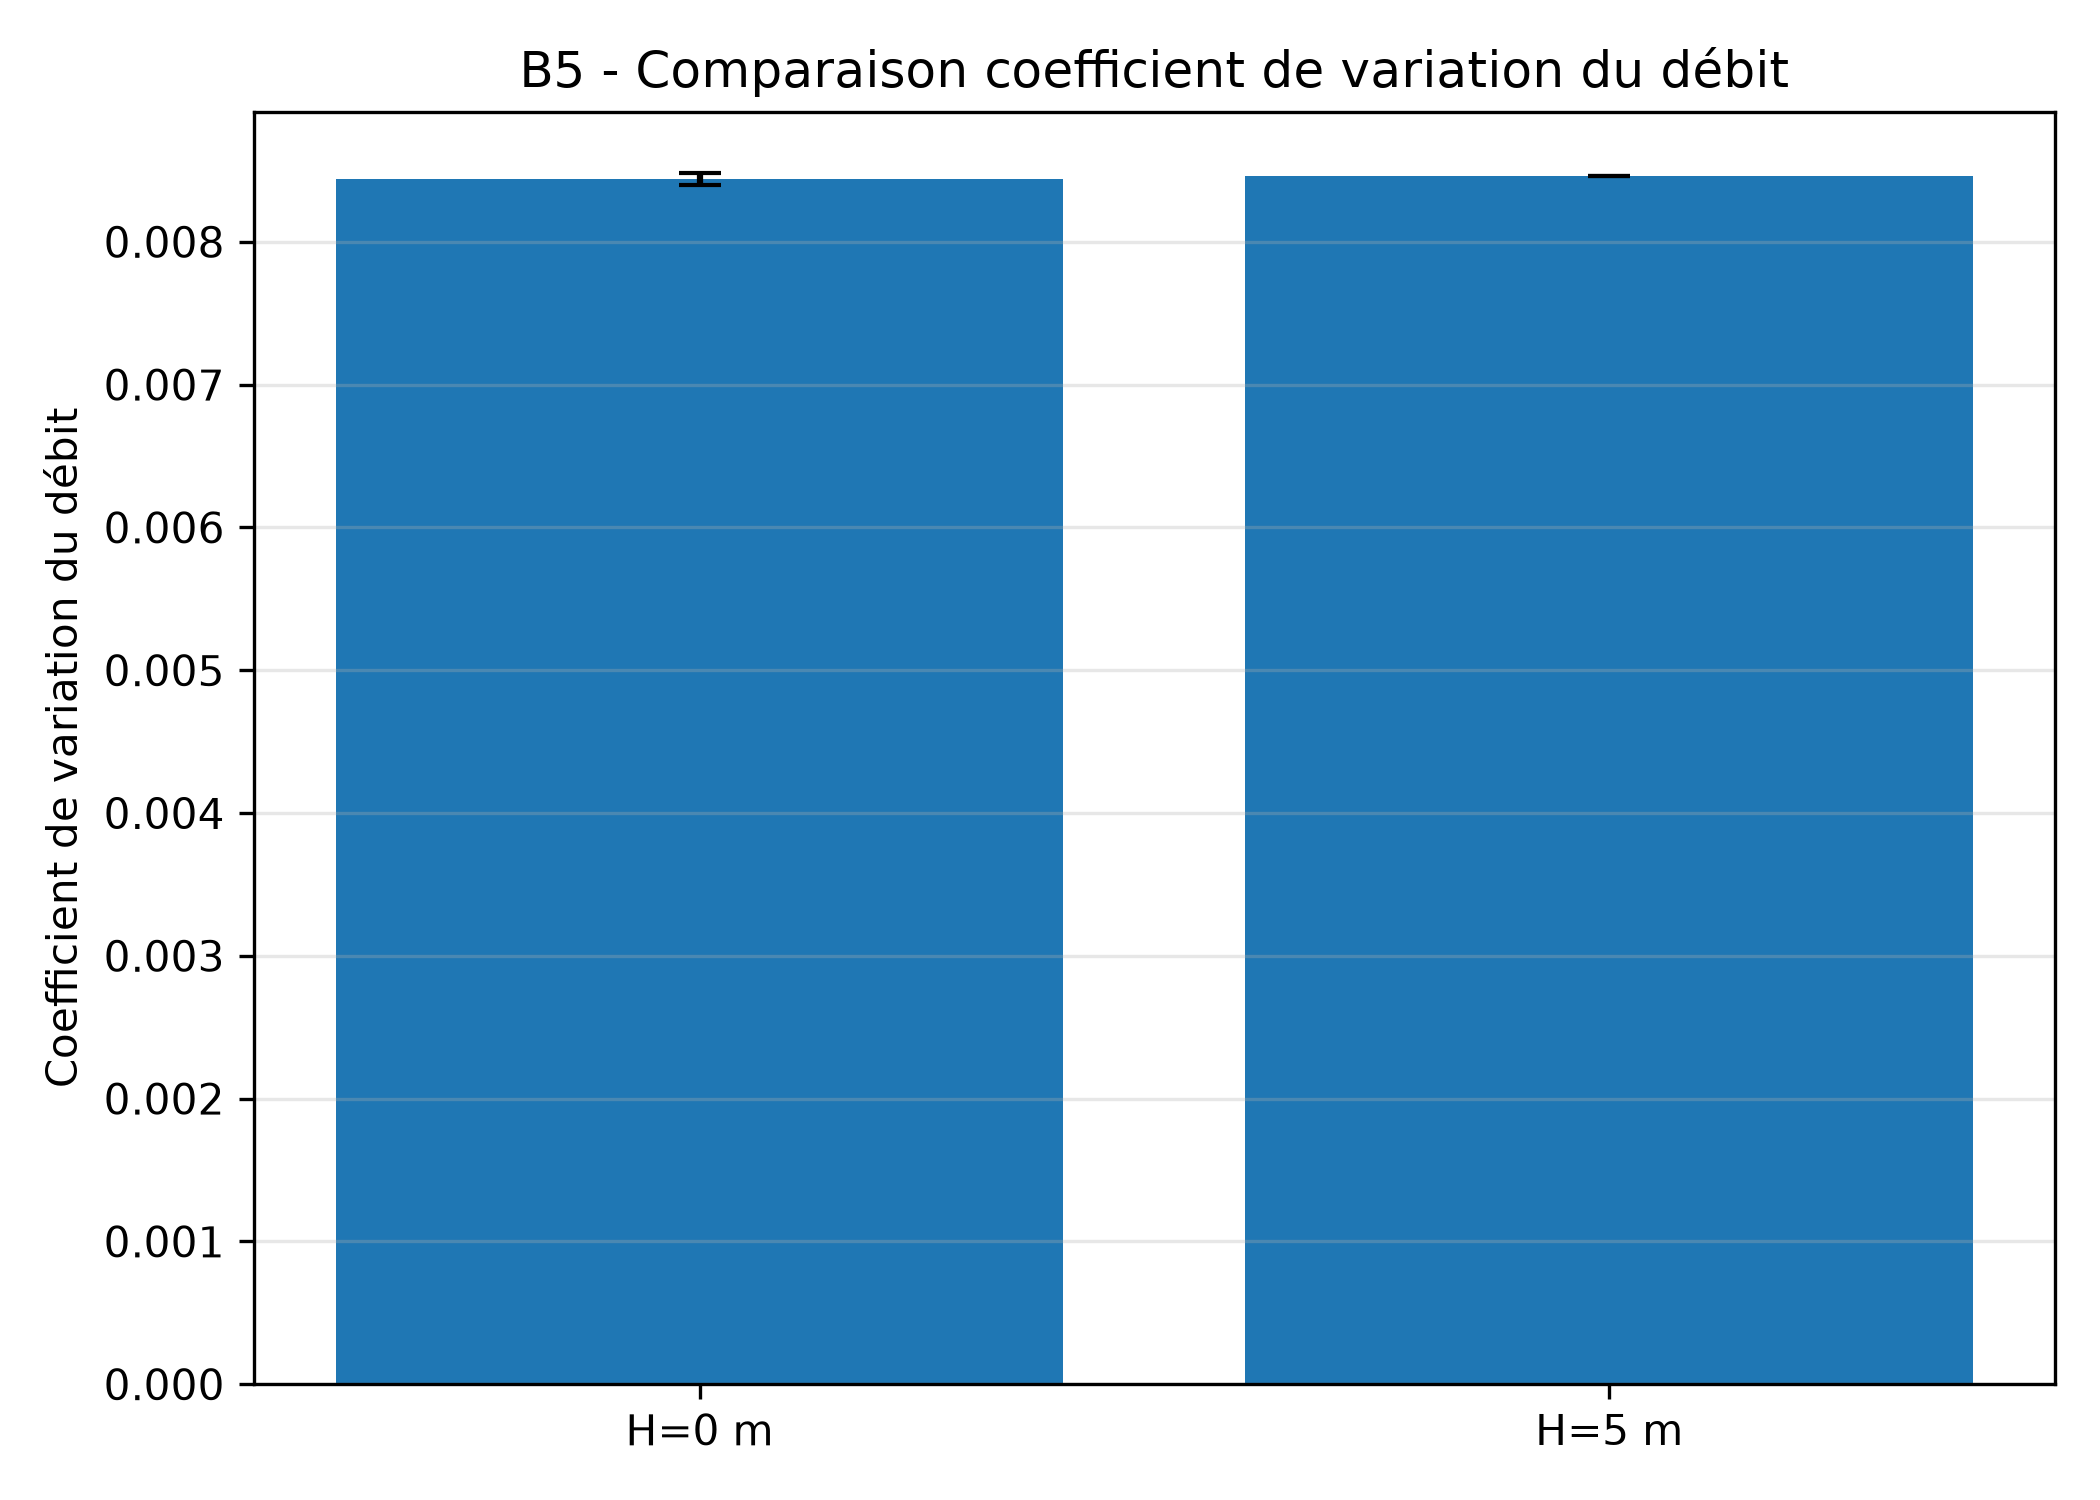
\includegraphics[width=0.85\textwidth]
    {img/B/B5_throughput_cv.png}
    \caption{Comparaison du coefficient de variation du débit reçu.}
    \label{fig:b5_cv}
\end{figure}

\subsubsection{Effet sur le trafic et les performances}

La proportion du volume reçu via Wi-Fi diminue
légèrement, passant de 51,28 \% à 50 \%.

Cette différence est cohérente avec le fait que l'UE
entre plus tard dans la couverture Wi-Fi et la quitte
plus tôt lorsque l'hystérésis est activée.

Le débit moyen reste égal au débit nominal de 2 Mbps
dans les deux configurations. Aucun paquet perdu ni
aucune interruption de service mesurée n'ont été
observés dans ces exécutions.

Le délai moyen augmente légèrement, passant de
9,184 ms à 9,397 ms, tandis que le délai maximal
reste identique à 22,731 ms.

% Figure 4 : Proportion du volume reçu via Wi-Fi
\begin{figure}[H]
    \centering
    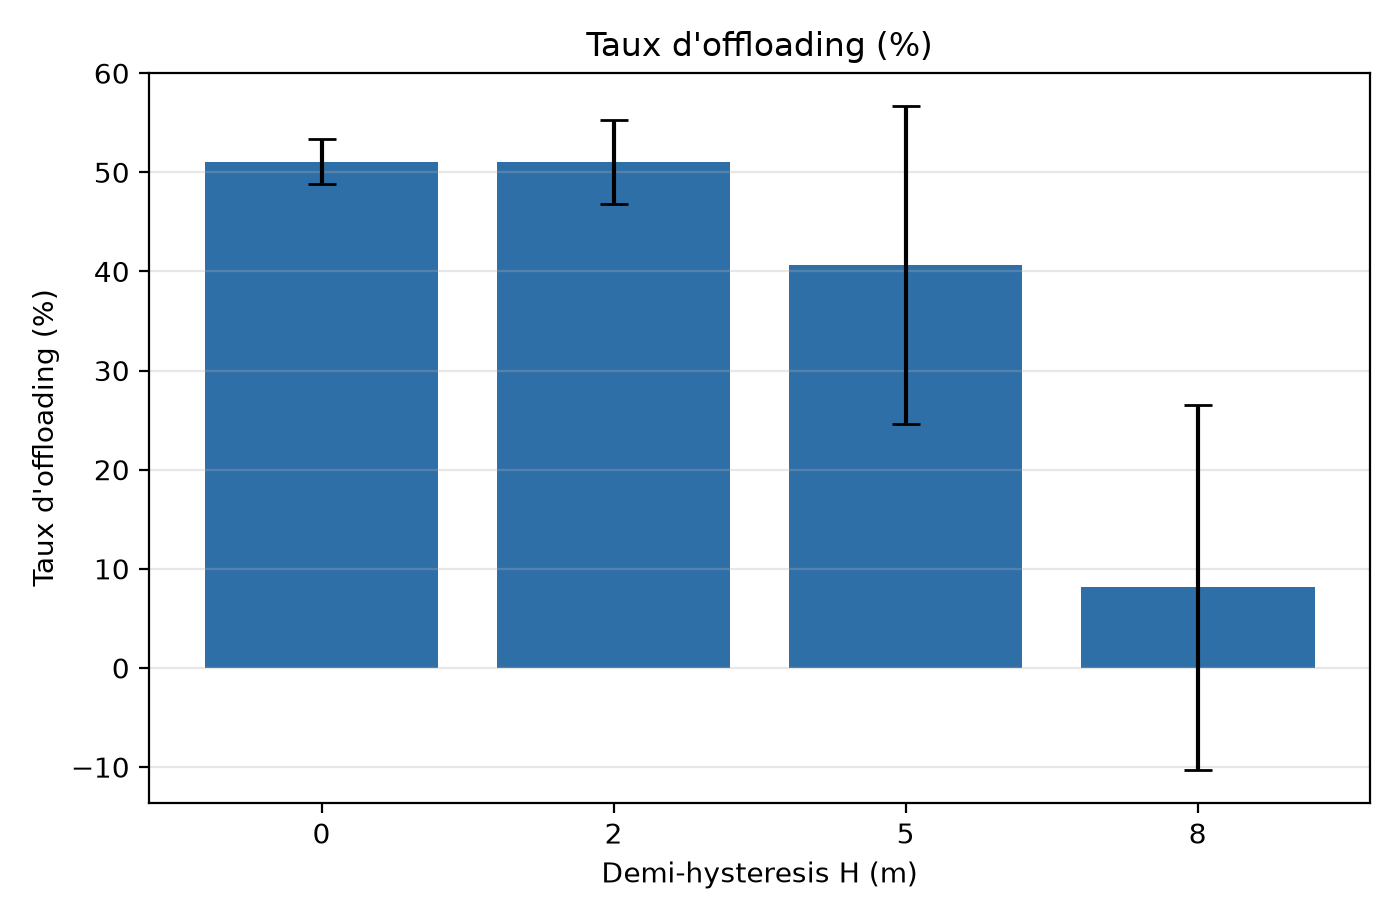
\includegraphics[width=0.85\textwidth]
    {img/B/B5_offloading.png}
    \caption{Comparaison de la proportion du volume reçu via Wi-Fi.}
    \label{fig:b5_offloading}
\end{figure}

\subsection{Discussion des résultats}

Les résultats montrent que l'introduction d'une
hystérésis permet de réduire le nombre de changements
d'interface lorsque l'UE se déplace à proximité de la
limite de couverture Wi-Fi.

Néanmoins, l'amélioration observée reste modeste :
le nombre total de bascules diminue de 5 \%, tandis
que le nombre d'événements de ping-pong diminue
d'environ 5,26 \%.

Par ailleurs, le coefficient de variation du débit
reste pratiquement identique entre les deux
configurations. L'hystérésis n'apporte donc pas,
dans ce scénario, de gain significatif en matière
de stabilité du débit.

Il faut également préciser que les cinq exécutions
utilisent la même graine initiale et que le shadowing
ainsi que le bruit sur la distance sont désactivés.
Les écarts-types nuls obtenus pour le nombre de
bascules et les événements de ping-pong traduisent
donc essentiellement la reproductibilité du scénario
déterministe. Ces exécutions ne constituent pas une
étude de la variabilité inter-graines.

\subsection{Conclusion}

Cette expérience a permis d'étudier l'influence de
l'hystérésis sur le mécanisme de bascule entre LTE
et Wi-Fi.

En introduisant deux seuils distincts, un seuil
d'entrée de 45 m et un seuil de sortie de 55 m,
le nombre moyen de bascules passe de 20 à 19,
soit une réduction de 5 \%.

Le nombre d'événements de ping-pong diminue
également, tandis que le débit moyen reste stable
à 2 Mbps. Cependant, le coefficient de variation
ne montre aucune amélioration notable de la
stabilité du débit.

Nous pouvons donc conclure que l'hystérésis
constitue un mécanisme pertinent pour limiter
les bascules répétées à proximité de la limite
de couverture, mais que son efficacité dépend
du scénario de mobilité et des paramètres choisis.
Dans le scénario étudié, son apport est réel
mais limité.

% ============================================================
% FIN DE LA QUESTION B5
% ============================================================
